% Format of Rendiconti di Matematica e delle sue Applicazioni (guidelines for authors, 10 October 2026):
% amsart 10pt, amsthm, hyperref, text body 12.5 x 19 cm, parindent 16pt; equation numbers on the right,
% as in the published articles of vol. 47 (2026).
\documentclass[10pt,reqno]{amsart}
\usepackage{amsthm,hyperref}
\setlength{\textwidth}{12.5cm}
\setlength{\textheight}{19cm}
\setlength{\parindent}{16pt}
\usepackage{amsmath,amssymb,graphicx,array,longtable,enumitem}

\hypersetup{colorlinks=true,linkcolor=blue,citecolor=blue,urlcolor=blue}
\hypersetup{pdftitle={An elementary-arithmetic splitting of the log-sine Mellin transform},pdfauthor={Victor Casana-Giner}}

\numberwithin{equation}{section}
\setlength{\emergencystretch}{1.5em}
\newtheorem{theorem}{Theorem}[section]
\newtheorem{lemma}[theorem]{Lemma}
\newtheorem{proposition}[theorem]{Proposition}
\newtheorem{corollary}[theorem]{Corollary}
\theoremstyle{definition}
\newtheorem{definition}[theorem]{Definition}
\theoremstyle{remark}
\newtheorem{remark}[theorem]{Remark}

\newcommand{\dd}{\,\mathrm{d}}
\newcommand{\Rez}{\operatorname{Re}}
\newcommand{\Imz}{\operatorname{Im}}
\newcommand{\Res}{\operatorname{Res}}

\title[Log-sine Mellin splitting]{An elementary--arithmetic splitting\\ of the log-sine Mellin transform}
\author{V\'ictor Casa\~na-Giner}
\address{Universidad Nacional de Educaci\'on a Distancia (UNED), Madrid, Spain}
\email{vcasana1@alumno.uned.es}
\urladdr{https://orcid.org/0000-0002-8252-2608}
\subjclass[2020]{11M06, 30B40, 44A15}
\keywords{sine product, log-sine constant, Mellin transform, Mittag-Leffler expansion, Riemann zeta function}

\begin{document}

\begin{abstract}
This work starts from the product $P(x)$ of the numbers $\sin(\pi x/k)$ over the integers $2\le k<x$, which is zero at the composite integers. We prove that $|P(p)|^{1/p}$ tends to $e^{-C_g}$ along the primes $p$, where $C_g=0.7437948618\ldots$ is a log-sine analogue of Euler's constant. The proof leads to two Mellin integrals of $h(u)=\log|2\sin\pi u|$: an arithmetic part $G(s)$, taken over $u>1$, and an elementary part $A(s)$, taken over $0<u<1$. Here $C_g=\log 2-G(1)$. We prove that $G$ is entire and $A$ meromorphic, with a Mittag-Leffler expansion whose coefficients are the values of the zeta function at the even integers; this gives $C_g$ in terms of these values. They satisfy $G(s)-A(s)=(\pi/s)\cot(\pi s/2)\,\zeta(s)$, so that a non-real $s$ is a zero of $\zeta$ if and only if $G(s)=A(s)$. We then study this identification of the zeros. A non-negative function $Q$ with $Q''=-h$ and $Q=Q'=0$ at the integers has a Mellin transform which is the sum of three terms: one given by $G$ and the other two, which nearly cancel, by $A$. Finally, deformations $h_b$ of $h$ keep such a function, and their parts $G_b$, $A_b$ are equal at infinitely many points on any prescribed finite set of vertical lines of the critical strip.
\end{abstract}
\maketitle

\section{Introduction}\label{sec:intro}

This work began with the study of the product
\[
P(x)=\prod_{2\le k<x}\sin\frac{\pi x}{k}\qquad(x\ge2),
\]
with the empty product $P(2)=1$. For an integer $x\ge2$ this product is zero exactly when $x$ is composite, so that its size at the primes is the natural quantity to study. Trigonometric analogues of trial division have been used in analytic prime indicators; see, for instance, Fuchs \cite{Fuchs2025}.

At the primes, $|P(p)|^{1/p}\to e^{-C_g}$ (Theorem~\ref{thm:Plimit}, Corollary~\ref{cor:Pdecay}), where
\[
C_g=-\int_0^1\log\sin\bigl(\pi\{1/v\}\bigr)\dd v=0.7437948618\ldots
\]
is a log-sine analogue of Euler's constant (Remark~\ref{rem:Euler}; sequence A402034 in the OEIS \cite{OEIS}).

The proof of this limit is what led to the functions studied in the rest of the paper. With
\begin{equation}\label{eq:h}
h(u)=\log|2\sin \pi u|,\qquad u\in\mathbb R\setminus\mathbb Z ,
\end{equation}
one has $\log\bigl(2^{p-2}|P(p)|\bigr)=\sum_{k=2}^{p-1}h(p/k)$. The points $u=p/k$ lie in $(1,\infty)$ with spacing about $u^2/p$, so that $\frac1p\sum_k h(p/k)$ is a Riemann sum for $\int_1^\infty h(u)u^{-2}\dd u$. This integral is the value at $s=1$ of the first of the two functions
\begin{equation}\label{eq:GA}
G(s)=\int_1^\infty h(u)\,u^{-s-1}\dd u,\qquad A(s)=-\int_0^1 h(u)\,u^{-s-1}\dd u ,
\end{equation}
and $C_g=\log 2-G(1)$. The integral for $G$ converges (as an improper integral) for $\Rez s>-1$, and the integral for $A$ for $\Rez s<0$; both functions are continued analytically below. The second function, $A$, is the same integral over the period $0<u<1$ that the product does not use.

The two functions satisfy
\[
G(s)-A(s)=\frac{\pi}{s}\cot\Bigl(\frac{\pi s}{2}\Bigr)\zeta(s)
\]
(Proposition~\ref{prop:D}), so that a non-real $s$ is a zero of $\zeta$ if and only if $G(s)=A(s)$.

The function $h$ is $1$-periodic and even, has logarithmic singularities at the integers, and has the Fourier expansion
\begin{equation}\label{eq:hfourier}
h(u)=-\sum_{n\ge1}\frac{\cos 2\pi n u}{n}\qquad (u\notin\mathbb Z),
\end{equation}
which follows from $\log|1-e^{2\pi i u}|=\Rez\log(1-e^{2\pi iu})$.

With $\theta=2\pi u$, it is the function $\log|2\sin(\theta/2)|$ whose integrals are the log-sine integrals and the Clausen function; see Lewin \cite{Lewin1981}, Zhang and Williams \cite{ZhangWilliams1995}, and Choi, Cho and Srivastava \cite{ChoiChoSrivastava2009}. Integrals involving it have a long history going back to Euler and form a substantial literature \cite{Onodera2011,BorweinStraub2012,Alkan2013,Umezawa2019,Shalev2025}; for $q$-analogues see Kurokawa, Mimachi and Wakayama \cite{KMW2007}, for incomplete Mellin transforms of related functions see Adam \cite{Adam2020}, and for background on Mellin transforms see Zagier \cite{Zagier2006}.

Here $h$ is integrated against $u^{-s-1}$ over the half-line, the integral is cut at $u=1$, the point given by the product $P$, and the two parts are studied as a pair $(G,A)$ of functions of $s$, each with properties of its own (Table~\ref{tab:GA}). We call $G$ the \emph{arithmetic part} and $A$ the \emph{elementary part}. The zeros of $\zeta$ are then given by the equality of two functions defined by explicit integrals, one of them continued meromorphically, which can be compared with each other.

\begin{table}[ht]
\centering
\begin{tabular}{>{\raggedright}p{0.21\textwidth}|>{\raggedright}p{0.33\textwidth}|>{\raggedright\arraybackslash}p{0.33\textwidth}}
 & $G(s)$ & $A(s)$\\
\hline
Interval & $1<u<\infty$ & $0<u<1$\\
Content & every singularity of $h$ at $u=1,2,3,\dots$ & one period, where $h$ is given by a power series\\
Continuation & entire (Corollary~\ref{cor:Gentire}) & meromorphic (Theorem~\ref{thm:ML})\\
Poles & none & double at $s=0$, simple at $s=2k$ with residue $-\zeta(2k)/k$\\
Explicit form & $G(1)=\log 2-C_g$, the limit along the primes (Theorem~\ref{thm:Plimit}) & series with coefficients $\zeta(2k)/k$ \eqref{eq:ML}\\
In the transform of $Q$ & the term from $u>1$ & the sum of the two terms from $u<1$
\end{tabular}
\caption{The two functions of the splitting.}\label{tab:GA}
\end{table}

Section~\ref{sec:product} contains the product and the constant $C_g$.

In Section~\ref{sec:GA} we derive the Mittag-Leffler expansion of $A$ (Theorem~\ref{thm:ML}) and prove the identity for $G-A$. As a consequence, $C_g$ has an expression in terms of the values $\zeta(2k)$ (Proposition~\ref{prop:Cg}). We also give the leading term of $A$ (Proposition~\ref{prop:Apsi}).

In Section~\ref{sec:Q} we consider the function $Q\ge0$ with $Q''=-h$ and $Q(n)=Q'(n)=0$ at the integers, and split its Mellin transform into three terms. The term from $u>1$ is given by $G$ and the other two by $A$. Each of these two is of order $|t|^{-1}$, and their sum is $O(|t|^{-3}\log|t|)$ because $Q(1)=Q'(1)=0$ (Theorem~\ref{thm:J}, Corollary~\ref{cor:T13}).

In Section~\ref{sec:def} we give functions $h_b$, obtained from $h$ by a dilation by a prime $p$, whose associated functions $Q_b$ keep $Q_b\ge0$, $Q_b''=-h_b$ and $Q_b(n)=Q_b'(n)=0$. They satisfy \eqref{eq:euler2} for $r$ prime to $p$, and $G_b=A_b$ at an infinite arithmetic progression of points on an arbitrary vertical line in $0<\Rez s<1$ (Theorem~\ref{thm:def}); the same holds simultaneously on any finite set of vertical lines (Theorem~\ref{thm:multi}). The relations \eqref{eq:euler2} for all $r$ determine $h$ up to a constant factor, and without the multiples of $p$ we classify the solutions and place the zeros (Proposition~\ref{prop:rigid}, Corollary~\ref{cor:place}). Consequently, such a function $Q_b$ together with \eqref{eq:euler2} for $r$ prime to one prime is not enough to show $G\ne A$ off a line (Remark~\ref{rem:nogo}).

Section~\ref{sec:num} gives the three terms of Section~\ref{sec:Q} at three heights, and Section~\ref{sec:notation} lists the symbols.

\smallskip
\noindent\textbf{Declaration on the use of AI.} During the preparation of this work, the author used Claude (Anthropic) as a tool for refining arguments, checking computations, and drafting and revising the manuscript. Every statement obtained with AI assistance has been reduced to elementary logical steps, each of which the author has checked and understood. In addition, the author has searched the literature by hand for every such statement, to avoid inadvertent plagiarism. The author takes full responsibility for the content of this paper.

\section{Notation}\label{sec:notation}
The symbols used in the paper, with the place where each is defined, are:

\smallskip
\begin{longtable}{@{}>{$}l<{$} p{0.62\textwidth}@{}}
h(u) & $\log|2\sin\pi u|$, \eqref{eq:h}\\
H(u) & $\int_1^u h$, bounded antiderivative of $h$\\
G(s),\ A(s) & arithmetic and elementary parts of the Mellin transform of $h$, \eqref{eq:GA}\\
a_k & $\zeta(2k)/k$, coefficients of \eqref{eq:ML}\\
k & summation index in \eqref{eq:hsmall}, \eqref{eq:ML}, \eqref{eq:A2}\\
r & multiplier in \eqref{eq:euler2}\\
j & index $j\ge2$ of the coefficients $b_j$; $m_j=2(j-1)$\\
n,\ m & positive integers in Fourier series\\
C_g & the log-sine constant $\log 2-G(1)=0.7437948618\ldots$, Definition~\ref{def:Cg}\\
P(x),\ x & the sine product \eqref{eq:P} and its real variable $x\ge2$\\
K(x),\ u_k,\ L & number of factors of $P(x)$, the points $x/k$, and the end of a fixed interval, Section~\ref{sec:product}\\
\varphi,\ \varphi_Y,\ F_Y,\ I_Y,\ E_Y & functions in the proof of Theorem~\ref{thm:Plimit}; $Y$ is the truncation level\\
d_k,\ \varepsilon,\ \omega,\ \delta,\ W_\omega,\ \rho,\ \Xi & quantities in Step 3 of the proof of Theorem~\ref{thm:Plimit}\\
\gamma & Euler's constant, Remark~\ref{rem:Euler} and Proposition~\ref{prop:Apsi}\\
U & random variable uniform on $(0,1)$\\
Q(u) & the function \eqref{eq:Q}; $Q''=-h$\\
q_0(u),\ c & singular part of $Q$ at $0$ and $c=\frac32-\log2\pi$, \eqref{eq:q0}\\
b_j & Taylor coefficients of $Q-q_0$, \eqref{eq:bj}\\
J,\ T_1,\ T_2,\ T_3 & Mellin moment of $Q$ and its three terms, \eqref{eq:T}, \eqref{eq:J}\\
s=\sigma+it & complex variable; $\sigma=\Rez s$, $t=\Imz s$\\
\tau_1 & imaginary part of the first zero of $\zeta$ in the upper half-plane\\
t_1 & $14.134725141734693790$, truncation of $\tau_1$ to $20$ digits\\
p,\ b,\ \sigma_0 & prime, deformation parameter in $(0,1)$, and $\log(1/b)/\log p$, Section~\ref{sec:def}\\
h_b,\ Q_b,\ G_b,\ A_b & deformed objects, \eqref{eq:hb}\\
B_p(s) & $\int_1^p h(u)u^{-s-1}\dd u$, Theorem~\ref{thm:def}(e)\\
D_p,\ E_p & $f\mapsto f(p\,\cdot)$ and $f\mapsto p^{-2}f(p\,\cdot)$, Theorem~\ref{thm:multi}\\
\sigma_j,\ \eta_j,\ \boldsymbol\eta,\ S,\ \eta_S & data of Theorem~\ref{thm:multi}; $M$ there is the number of lines\\
\psi & $\Gamma'/\Gamma$, Proposition~\ref{prop:Apsi}\\
\kappa_n,\ F,\ F_N,\ f_N & coefficients, antiderivative and partial sums in Lemma~\ref{lem:termwise}\\
R_\beta & radius of convergence of $\sum_\nu\beta_\nu z^\nu$, Proposition~\ref{prop:rigid}(c)\\
\ell & integer index of the points in Theorem~\ref{thm:def}(d) and Corollary~\ref{cor:place}\\
\lambda & constant factor in Proposition~\ref{prop:rigid}(a)\\
f,\ \hat f(n) & real even periodic function and its Fourier coefficients, Proposition~\ref{prop:rigid}\\
G_f,\ A_f & \eqref{eq:GA} with $f$ in place of $h$\\
v_p(n) & exponent of $p$ in $n$\\
\beta_\nu,\ \nu & coefficient sequence in \eqref{eq:fbeta} and its index\\
\Phi_\beta,\ z & the power series in \eqref{eq:Phibeta} and its variable\\
z_i,\ M,\ \Phi,\ \mu & data of Corollary~\ref{cor:place}\\
\theta & variable of the classical kernel $\log|2\sin(\theta/2)|$\\
y,\ v,\ w & integration variables\\
\end{longtable}
\addtocounter{table}{-1}


\section{The sine product and the constant \texorpdfstring{$C_g$}{Cg}}\label{sec:product}

\subsection{The product}

For real $x\ge2$ let
\begin{equation}\label{eq:P}
P(x)=\prod_{2\le k<x}\sin\frac{\pi x}{k},
\end{equation}
the empty product being $1$; in particular $P(2)=1$.

\begin{proposition}\label{prop:Pzero}
Let $x\ge2$ be an integer. Then $P(x)=0$ if and only if $x$ is composite.
\end{proposition}

\begin{proof}
The factor with index $k$ is zero if and only if $k\mid x$.

An integer $k$ with $2\le k<x$ and $k\mid x$ exists if and only if $x$ is composite.
\end{proof}

Since $|2\sin\pi u|=e^{h(u)}$, for every $x\ge2$ with $P(x)\ne0$,
\begin{equation}\label{eq:logP}
\log\Bigl(2^{K(x)}|P(x)|\Bigr)=\sum_{2\le k<x}h\Bigl(\frac xk\Bigr),
\end{equation}
where $K(x)$ is the number of factors in \eqref{eq:P}.

The points $u_k=x/k$ decrease as $k$ increases, all of them exceed $1$, and
\[
u_k-u_{k+1}=\frac{u_ku_{k+1}}{x}.
\]
Hence
\begin{equation}\label{eq:Riemann}
\frac1x\sum_{2\le k<x}h(u_k)=\sum_{2\le k<x}\frac{h(u_k)}{u_ku_{k+1}}\,(u_k-u_{k+1}).
\end{equation}

On each fixed interval $1<u\le L$ the points $u_k$ have spacing at most $L^2/x$, so that there the right-hand side of \eqref{eq:Riemann} has the form of a Riemann sum for $\int h(u)u^{-2}\dd u$. The integral of $h(u)u^{-2}$ over the whole range $u>1$ is $G(1)$. Because $h$ has logarithmic singularities at the integers, the convergence of these sums needs a proof; at the primes it holds.

\begin{theorem}\label{thm:Plimit}
As $p\to\infty$ through the primes,
\begin{equation}\label{eq:Plimit}
\frac1p\sum_{k=2}^{p-1}h\Bigl(\frac pk\Bigr)=\frac1p\log\Bigl(2^{p-2}|P(p)|\Bigr)\longrightarrow G(1)=\int_1^\infty\frac{h(u)}{u^2}\dd u .
\end{equation}
\end{theorem}

\begin{proof}
Let $\varphi(t)=h(t)$ for $0<t<1$, so that $h(y)=\varphi(\{y\})$ for $y\notin\mathbb Z$. For $p$ prime and $2\le k<p$ we have $k\nmid p$, so $\{p/k\}\in(0,1)$ and $h(p/k)=\varphi(\{p/k\})$.

\emph{Step 1: truncation.} For $Y>0$ put $\varphi_Y=\max(\varphi,-Y)$, extended by $\varphi_Y(0)=\varphi_Y(1)=-Y$. Since $\varphi\le\log2$ and $\varphi(t)\to-\infty$ as $t\to0^+$ or $t\to1^-$, the function $\varphi_Y$ is continuous on $[0,1]$, and $F_Y(v)=\varphi_Y(\{1/v\})$ is bounded on $(0,1]$ and continuous there (at $v=1/m$ both one-sided limits equal $-Y$). Hence $F_Y$ is Riemann integrable on $[0,1]$, and its Riemann sums with the points $k/p$ converge:
\[
\frac1p\sum_{k=2}^{p-1}\varphi_Y\Bigl(\Bigl\{\frac pk\Bigr\}\Bigr)=\frac1p\sum_{k=2}^{p-1}F_Y\Bigl(\frac kp\Bigr)\longrightarrow I_Y:=\int_0^1F_Y(v)\dd v,
\]
the two omitted terms $k=1,p$ contributing $O(Y/p)$.

\emph{Step 2: the limit of $I_Y$.} With $u=1/v$, $G(1)=\int_0^1h(1/v)\dd v=\int_0^1\varphi(\{1/v\})\dd v$, and this integral converges absolutely because $\int_1^\infty|h(u)|u^{-2}\dd u<\infty$. As $Y\to\infty$, $F_Y$ decreases to $F(v):=\varphi(\{1/v\})$ and $F_Y\le\log2$. Apply the monotone convergence theorem to the nonnegative increasing functions $\log2-F_Y\uparrow\log2-F$: this gives $\int_0^1(\log2-F_Y)\to\int_0^1(\log2-F)$, i.e.\ $I_Y\to G(1)$.

\emph{Step 3: the error near the singularities.} Let $d_k=\operatorname{dist}(p/k,\mathbb Z)$. Since $|\sin\pi y|\ge2\operatorname{dist}(y,\mathbb Z)$, we have $h(p/k)\ge\log(4d_k)$, hence
\[
0\le\varphi_Y(\{p/k\})-h(p/k)\le\log\frac1{4d_k}\cdot\mathbf 1\bigl[4d_k<e^{-Y}\bigr].
\]
Let $\omega\ge1$ be the integer nearest to $p/k$ and $\delta=|p-\omega k|$, so that $d_k=\delta/k$ and $\delta\ge1$ because $k\nmid p$. For fixed $\omega$, the integers $k$ with nearest integer $\omega$ lie in $\bigl[p/(\omega+\frac12),p/(\omega-\frac12)\bigr]$, so $k\le W_\omega:=2p/\omega$, and the numbers $p-\omega k$ for these $k$ form an arithmetic progression of difference $\omega$. Put $\varepsilon=e^{-Y}/4$. The condition $4d_k<e^{-Y}$ gives $\delta<\varepsilon k\le\varepsilon W_\omega$; it is impossible unless $\omega\le2\varepsilon p$. Among the terms of the progression in $(0,\varepsilon W_\omega)$, the $\rho$-th smallest is $\ge1+(\rho-1)\omega$, and the same holds in $(-\varepsilon W_\omega,0)$. Since $\log(k/(4\delta))\le\log(W_\omega/\delta)$ and $y\mapsto\log(W_\omega/y)$ is decreasing,
\[
\begin{aligned}
\sum_{k:\,\mathrm{nearest}=\omega}\log\frac{1}{4d_k}\,\mathbf 1\bigl[4d_k<e^{-Y}\bigr]
&\le2\Bigl(\log W_\omega+\frac1\omega\int_0^{\varepsilon W_\omega}\log\frac{W_\omega}{y}\dd y\Bigr)\mathbf 1[\omega\le2\varepsilon p]\\
&\le2\log\frac{2p}\omega\,\mathbf 1[\omega\le2\varepsilon p]+\frac{4\varepsilon p}{\omega^2}\Bigl(\log\frac1\varepsilon+1\Bigr).
\end{aligned}
\]
Summing over $\omega$ and using $\sum_{\omega\le \Xi}\log(2p/\omega)\le\int_0^\Xi\log(2p/y)\dd y=\Xi(\log(2p/\Xi)+1)$ with $\Xi=2\varepsilon p$,
\[
E_Y(p):=\frac1p\sum_{k=2}^{p-1}\bigl(\varphi_Y(\{p/k\})-h(p/k)\bigr)\le4\varepsilon\Bigl(\log\frac1\varepsilon+1\Bigr)\bigl(1+\zeta(2)\bigr),
\]
uniformly in $p$; the right-hand side tends to $0$ as $Y\to\infty$.

\emph{Step 4: conclusion.} By Steps 1 and 3,
\[
I_Y-\sup_pE_Y(p)\le\liminf_{p}\frac1p\sum_{k=2}^{p-1}h\Bigl(\frac pk\Bigr)\le\limsup_{p}\frac1p\sum_{k=2}^{p-1}h\Bigl(\frac pk\Bigr)\le I_Y .
\]
Letting $Y\to\infty$ and using Steps 2 and 3 gives \eqref{eq:Plimit}. The equality in \eqref{eq:Plimit} is \eqref{eq:logP}, with $K(p)=p-2$.
\end{proof}

This is how the function $G$ enters.

\subsection{The constant \texorpdfstring{$C_g$}{Cg}}

\begin{definition}\label{def:Cg}
The log-sine constant is
\[
C_g:=\log 2-G(1)=\log2-\int_1^\infty\frac{h(u)}{u^2}\dd u .
\]
\end{definition}

\begin{proposition}\label{prop:Cg}
\begin{enumerate}[label=(\alph*)]
\item With $\{\cdot\}$ the fractional part and $U$ uniform on $(0,1)$,
\begin{equation}\label{eq:Cg}
C_g=-\int_0^1\log\sin\bigl(\pi\{1/v\}\bigr)\dd v=-\mathbb E\,\log\sin\bigl(\pi\{1/U\}\bigr).
\end{equation}
\item In terms of the values $\zeta(2k)$,
\begin{equation}\label{eq:Cgzeta}
C_g=\log 2+\frac{\pi^2}{2}-\log 2\pi-1-\sum_{k\ge1}\frac{\zeta(2k)}{k(2k-1)}=0.7437948618\ldots .
\end{equation}
\end{enumerate}
\end{proposition}

\begin{proof}[Proof of \textup{(a)}]
Put $u=1/v$ in $G(1)$. Then $G(1)=\int_0^1h(1/v)\dd v$.

By the periodicity of $h$ and $\sin(\pi\{y\})=|\sin\pi y|$, we have $h(1/v)=\log 2+\log\sin(\pi\{1/v\})$.
\end{proof}

Part (b) is proved in Section~\ref{sec:GA}, after Proposition~\ref{prop:D}.

\begin{corollary}\label{cor:Pdecay}
As $p\to\infty$ through the primes, $|P(p)|^{1/p}\to e^{-C_g}=0.4753\ldots$.
\end{corollary}

\begin{proof}
By Theorem~\ref{thm:Plimit}, $\frac1p\log|P(p)|=\frac1p\sum_{k=2}^{p-1}h(p/k)-\frac{p-2}p\log2\to G(1)-\log2=-C_g$.
\end{proof}

The decimal expansion of $C_g$ has been allocated the sequence number A402034 in the On-Line Encyclopedia of Integer Sequences \cite{OEIS}.

\begin{remark}\label{rem:Euler}
Formula \eqref{eq:Cg} is the log-sine analogue of the classical formula
\[
1-\gamma=\int_0^1\{1/v\}\dd v
\]
for Euler's constant $\gamma$: the fractional part $\{1/v\}$ is replaced by $-\log\sin(\pi\{1/v\})$.
\end{remark}

\section{The functions \texorpdfstring{$h$}{h}, \texorpdfstring{$G$}{G} and \texorpdfstring{$A$}{A}}\label{sec:GA}

\subsection{Two structural facts on \texorpdfstring{$h$}{h}}
For every integer $r\ge1$,
\begin{equation}\label{eq:euler2}
h(ru)=\sum_{j=0}^{r-1}h\Bigl(u+\frac jr\Bigr)\qquad(ru\notin\mathbb Z).
\end{equation}
These are the Kubert identities of exponent $1$ (exponent $s=1$ in Milnor's notation, not to be confused with our variable $s$); see Milnor \cite{Milnor1983}, Koblitz \cite{Koblitz1983}, Kanemitsu and Yoshimoto \cite{KanemitsuYoshimoto1996}, Porubsk\'y \cite{Porubsky2000}, and Lagarias and Li \cite{LagariasLi2016}.

Indeed $\sum_{j=0}^{r-1}\cos 2\pi n(u+j/r)$ equals $r\cos 2\pi nu$ if $r\mid n$ and $0$ otherwise, so by \eqref{eq:hfourier} the right-hand side is $-\sum_{m\ge1}r\cos(2\pi mr u)/(mr)=h(ru)$.

This identity of Fourier series holds in $L^2(0,1)$, hence almost everywhere; both sides are continuous on $\{u:\ ru\notin\mathbb Z\}$, so the equality holds at every point of that set.

For $|u|<1$, $u\neq0$, the product $\sin\pi u=\pi u\prod_{n\ge1}(1-u^2/n^2)$ \cite[\S3.23, p.~114]{Titchmarsh1939} gives
\begin{equation}\label{eq:hsmall}
h(u)=\log(2\pi|u|)-\sum_{k\ge1}\frac{\zeta(2k)}{k}\,u^{2k},
\end{equation}
after expanding $\log(1-u^2/n^2)$ and summing over $n$ (all terms are negative, so the order of summation is free).

\subsection{The arithmetic part}
Since $h$ is $1$-periodic with mean zero, $H(u)=\int_1^u h$ is bounded (it is $1$-periodic and continuous). Integrating by parts in \eqref{eq:GA},
\[
G(s)=(s+1)\int_1^\infty H(u)\,u^{-s-2}\dd u ,
\]
so $G$ is holomorphic in $\Rez s>-1$.

\subsection{The elementary part}

\begin{theorem}[Mittag-Leffler form of $A$]\label{thm:ML}
The integral defining $A$ converges for $\Rez s<0$, and $A$ extends to a meromorphic function on $\mathbb C$ given by
\begin{equation}\label{eq:ML}
A(s)=\frac{\log 2\pi}{s}+\frac1{s^2}+\sum_{k\ge1}\frac{a_k}{2k-s},\qquad a_k=\frac{\zeta(2k)}{k}.
\end{equation}
The series converges absolutely and locally uniformly off $\{2,4,6,\dots\}$. The poles of $A$ are a double pole at $s=0$ with principal part $1/s^2+\log(2\pi)/s$ and simple poles at $s=2k$ with residue $-a_k$. The numbers $a_k$ are rational multiples of $\pi^{2k}$ \cite{Patri2013}.
\end{theorem}

\begin{proof}
Near $u=0$, $h(u)=\log u+O(1)$, so the integral converges for $\Rez s<0$. Insert \eqref{eq:hsmall} into \eqref{eq:GA}. For $\Rez s<0$,
\[
\begin{split}
-\int_0^1 \log(2\pi)\,u^{-s-1}\dd u&=\frac{\log 2\pi}{s},\qquad
-\int_0^1 \log u\;u^{-s-1}\dd u=\frac1{s^2},\\
\int_0^1 u^{2k-s-1}\dd u&=\frac1{2k-s}.
\end{split}
\]
The interchange of sum and integral is justified by Tonelli's theorem applied to the absolute values: with $\sigma=\Rez s<0$,
\[
\sum_{k\ge1}a_k\int_0^1 \bigl|u^{2k-s-1}\bigr|\dd u=\sum_{k\ge1}\frac{a_k}{2k-\sigma}<\infty ,
\]
because $0<a_k\le\zeta(2)/k$; hence the series $\sum_k a_k u^{2k}u^{-s-1}$ converges absolutely in $L^1(0,1)$ and may be integrated term by term (Fubini).

This gives \eqref{eq:ML} for $\Rez s<0$. The right-hand side of \eqref{eq:ML} is meromorphic on $\mathbb C$, since $\sum_k |a_k|/|2k-s|$ converges locally uniformly off the even integers, and it provides the continuation.
\end{proof}

\begin{lemma}\label{lem:sum}
For $s=\sigma+it$ with $-1\le\sigma\le\frac32$ and $|t|\ge1$,
\[
\sum_{k\ge1}\frac{1}{k\,|2k-s|}\le\frac{3+\log|t|}{|t|}.
\]
\end{lemma}

\begin{proof}
We have $|2k-s|\ge|t|$ for every $k$, and $|2k-s|\ge 2k-\sigma\ge 2k-\frac32\ge k$ for $k\ge2$. Since $|t|\ge1$, the terms with $k\le|t|$ (among them $k=1$) contribute at most $|t|^{-1}\sum_{k\le|t|}k^{-1}\le(1+\log|t|)/|t|$, and the terms with $k>|t|$, all with $k\ge2$, contribute at most $\sum_{k>|t|}k^{-2}\le 2/|t|$.
\end{proof}

\begin{remark}\label{rem:Aelem}
The only arithmetic quantities in \eqref{eq:ML} are the values $\zeta(2k)$, i.e.\ the Taylor coefficients of $\log(\sin\pi u/\pi u)$; the poles, residues and growth of $A$ are known explicitly. For instance, uniformly in $-1\le\Rez s\le 3/2$, $|\Imz s|\ge1$,
\begin{equation*}
A(s)\ll \frac{1}{|s|}+\sum_{k\ge1}\frac{1}{k\,|2k-s|}\ll \frac{\log(|\Imz s|+2)}{|\Imz s|}
\end{equation*}
by \eqref{eq:ML}, $a_k\le\zeta(2)/k$ and Lemma~\ref{lem:sum}.
\end{remark}

The leading term of $A$ can be given explicitly. Let $\psi=\Gamma'/\Gamma$ and let $\gamma$ be Euler's constant.

\begin{proposition}\label{prop:Apsi}
For $s\notin\{0,2,4,6,\dots\}$,
\begin{equation}\label{eq:Apsi}
A(s)=\frac{\log\pi-\gamma-\psi(1-s/2)}{s}+\frac1{s^2}+\frac2s\sum_{k\ge1}\frac{\zeta(2k)-1}{2k-s},
\end{equation}
where the last series converges geometrically. Consequently, uniformly in $-1\le\Rez s\le\frac32$, $|\Imz s|\ge1$, with the principal branch of the logarithm,
\begin{equation}\label{eq:Aasym}
A(s)=\frac{\log 2\pi-\gamma-\log(-s)}{s}+O\Bigl(\frac1{|\Imz s|^{2}}\Bigr),
\end{equation}
and therefore
\[
T_1(s)+T_3(s)=\frac{\log 2\pi-\gamma-\log(-s)}{s(s+1)(s+2)}+O\Bigl(\frac1{|\Imz s|^{4}}\Bigr)
\]
with $T_1$, $T_3$ as in Section~\ref{sec:Q}.
\end{proposition}

\begin{proof}
Since $\frac{1}{k(2k-s)}=\frac1s\bigl(\frac{2}{2k-s}-\frac1k\bigr)$, \eqref{eq:ML} gives
\[
A(s)=\frac{\log2\pi}{s}+\frac1{s^2}+\frac1s\sum_{k\ge1}\zeta(2k)\Bigl(\frac{2}{2k-s}-\frac1k\Bigr).
\]
Write $\zeta(2k)=1+(\zeta(2k)-1)$.

For the part with $1$, the series $\psi(1+z)=-\gamma+\sum_{k\ge1}\bigl(\frac1k-\frac1{k+z}\bigr)$ \cite[Ch.~2, Ex.~2.2, p.~39]{Olver1997} with $z=-s/2$ gives $\sum_{k\ge1}\bigl(\frac2{2k-s}-\frac1k\bigr)=-\gamma-\psi(1-s/2)$.

For the other part,
\[
\sum_{k\ge1}\frac{\zeta(2k)-1}{k}=\sum_{n\ge2}\sum_{k\ge1}\frac{n^{-2k}}{k}=-\sum_{n\ge2}\log(1-n^{-2})=\log2,
\]
because $\prod_{n=2}^{N}(1-n^{-2})=\frac{N+1}{2N}\to\frac12$.

Adding up gives \eqref{eq:Apsi}. The series in \eqref{eq:Apsi} converges geometrically because $0<\zeta(2k)-1\le 2^{-2k}+\int_2^\infty x^{-2k}\dd x\le 3\cdot 2^{-2k}$ for $k\ge1$.

For \eqref{eq:Aasym}, put $w=1-s/2$; then $\Rez w\ge\frac14$, and $\psi(w)=\log w+O(1/|w|)$ there \cite[(5.11.2)]{DLMF}. Moreover $\log w=\log(-s/2)+\log(1-2/s)=\log(-s)-\log 2+O(1/|s|)$. The term $1/s^2$ is $O(|\Imz s|^{-2})$, and the last term of \eqref{eq:Apsi} is at most $\frac{2}{|s|\,|\Imz s|}\sum_k(\zeta(2k)-1)=O(|\Imz s|^{-2})$, since $|2k-s|\ge|\Imz s|$. The statement on $T_1+T_3$ follows from \eqref{eq:T13}.
\end{proof}

\subsection{The difference}

\begin{lemma}\label{lem:termwise}
Let $f(u)=-\sum_{n\ge1}\kappa_n\cos(2\pi nu)/n$ with real $\kappa_n$ and $\sum_n\kappa_n^2n^{-2}<\infty$, and let $F(u)=\int_1^u f$. Then $F(u)=-\sum_n\kappa_n\sin(2\pi nu)/(2\pi n^2)$ is continuous and bounded, the integral $\int_1^\infty f(u)u^{-s-1}\dd u:=(s+1)\int_1^\infty F(u)u^{-s-2}\dd u$ converges for $\Rez s>-1$, and $\int_0^1 f(u)u^{-s-1}\dd u$ converges absolutely for $\Rez s<-\frac12$. If $-1<\Rez s<-\frac12$, then the series below converges absolutely and
\begin{equation}\label{eq:termwise}
\int_0^1 f(u)u^{-s-1}\dd u+\int_1^\infty f(u)u^{-s-1}\dd u=-(2\pi)^s\Gamma(-s)\cos\Bigl(\frac{\pi s}2\Bigr)\sum_{n\ge1}\kappa_n n^{s-1}.
\end{equation}
\end{lemma}

\begin{proof}
By Cauchy--Schwarz, $\sum_n|\kappa_n|n^{-2}\le(\sum_n\kappa_n^2n^{-2})^{1/2}\zeta(2)^{1/2}<\infty$ and, for $\sigma=\Rez s<-\frac12$, $\sum_n|\kappa_n|n^{\sigma-1}\le(\sum_n\kappa_n^2n^{-2})^{1/2}(\sum_nn^{2\sigma})^{1/2}<\infty$; so the sine series for $F$ converges uniformly, and it represents the absolutely continuous primitive $F(u)=\int_1^uf(v)\dd v$: indeed $F_N(u)=\int_1^uf_N(v)\dd v$ for the partial sums $f_N$, $F_N$ with $n\le N$ (because $\sin2\pi n=0$), and $f_N\to f$ in $L^2$ of every bounded interval, hence in $L^1$ there, so that $\int_1^uf_N\to\int_1^uf$ locally uniformly in $u$.

Since $F$ is bounded, $\int_1^X fu^{-s-1}=F(X)X^{-s-1}+(s+1)\int_1^XFu^{-s-2}$ has a limit as $X\to\infty$ for $\Rez s>-1$. On $(0,1)$, $f\in L^2(0,1)$ and $u^{-s-1}\in L^2(0,1)$ for $\Rez s<-\frac12$.

For each $N$, by \eqref{eq:cosmellin} with $y=2\pi nu$, the left-hand side of \eqref{eq:termwise} for $f_N$ equals
\[
-(2\pi)^s\Gamma(-s)\cos\Bigl(\frac{\pi s}2\Bigr)\sum_{n\le N}\kappa_nn^{s-1}.
\]
As $N\to\infty$: $f_N\to f$ in $L^2(0,1)$, which gives convergence of the integral over $(0,1)$; $F_N\to F$ uniformly, which gives convergence of $(s+1)\int_1^\infty F_Nu^{-s-2}$; and the finite sums converge to the absolutely convergent series.
\end{proof}

\begin{proposition}\label{prop:D}
As an identity of meromorphic functions in $\Rez s>-1$,
\begin{equation}\label{eq:D}
G(s)-A(s)=\frac{\pi}{s}\cot\Bigl(\frac{\pi s}2\Bigr)\,\zeta(s).
\end{equation}
In particular both sides are finite and equal at every $s$ with $\Rez s>-1$, $s\notin\{0,2,4,6,\dots\}$. Consequently, for $s$ with $\Imz s\ne0$ and $\Rez s>-1$: $\zeta(s)=0$ if and only if $G(s)=A(s)$.
\end{proposition}

\begin{proof}
For $-1<\Rez s<0$ both integrals in \eqref{eq:GA} converge, and $G(s)-A(s)$ is the left-hand side of \eqref{eq:termwise} for $f=h$. From $\int_0^\infty y^{w-1}e^{\pm iy}\dd y=\Gamma(w)e^{\pm i\pi w/2}$ for $0<\Rez w<1$ (rotation of the path in Euler's integral for $\Gamma$), averaging the two signs and putting $w=-s$ (see also \cite[Part~I, \S1.5]{Oberhettinger1974}),
\begin{equation}\label{eq:cosmellin}
\int_0^\infty y^{-s-1}\cos y\dd y=\Gamma(-s)\cos\Bigl(\frac{\pi s}2\Bigr),\qquad -1<\Rez s<0 .
\end{equation}
Lemma~\ref{lem:termwise} with $\kappa_n=1$ gives, for $-1<\Rez s<-\frac12$,
\[
G(s)-A(s)=-\sum_{n\ge1}\frac{(2\pi n)^s}{n}\,\Gamma(-s)\cos\Bigl(\frac{\pi s}2\Bigr)=-(2\pi)^s\Gamma(-s)\cos\Bigl(\frac{\pi s}2\Bigr)\zeta(1-s).
\]
By the functional equation $\zeta(s)=2^s\pi^{s-1}\sin(\pi s/2)\Gamma(1-s)\zeta(1-s)$ \cite[Theorem~2.1, (2.1.1), p.~13]{TitchmarshHB1986} and $\Gamma(1-s)=-s\Gamma(-s)$, we have $(2\pi)^s\Gamma(-s)\zeta(1-s)=-\pi\zeta(s)/(s\sin(\pi s/2))$, which gives \eqref{eq:D} for $-1<\Rez s<-\frac12$; both sides are meromorphic in $\Rez s>-1$, so \eqref{eq:D} holds there as an identity of meromorphic functions; the poles of both sides are $s=0$ and $s=2,4,6,\dots$ (Remark~\ref{rem:poles}).

For $\Imz s\ne0$, $\cot(\pi s/2)$ is finite and nonzero and $s\neq0$, which gives the last assertion.
\end{proof}

\begin{remark}\label{rem:poles}
The poles of the two sides of \eqref{eq:D} match: at $s=0$, $\cot(\pi s/2)=2/(\pi s)+O(s)$, $\zeta(0)=-\frac12$ and $\zeta'(0)=-\frac12\log2\pi$ give the principal part $-1/s^2-\log(2\pi)/s$, which is that of $-A$; at $s=2k$ the residue of the right-hand side is $(\pi/2k)(2/\pi)\zeta(2k)=a_k$, which is the residue of $-A$.

The arithmetic part $G$ is regular at all these points. At $s=1$, the zero of $\cot(\pi s/2)$ cancels the pole of $\zeta$:
\begin{equation}\label{eq:G1}
G(1)=A(1)-\frac{\pi^2}{2},\qquad A(1)=\log 2\pi+1+\sum_{k\ge1}\frac{\zeta(2k)}{k(2k-1)} .
\end{equation}
\end{remark}

This cancellation of poles also shows the following.

\begin{corollary}\label{cor:Gentire}
$G$ extends to an entire function, and $G(-1)=A(-1)=0$. Consequently \eqref{eq:D} holds on $\mathbb C$ as an identity of meromorphic functions, and for every non-real $s$: $\zeta(s)=0$ if and only if $G(s)=A(s)$.
\end{corollary}

\begin{proof}
By Proposition~\ref{prop:D}, $G=A+(\pi/s)\cot(\pi s/2)\zeta(s)$, and the right-hand side is meromorphic on $\mathbb C$.

Its possible poles are those of $A$, at $s=0$ and $s=2,4,6,\dots$, and those of $(\pi/s)\cot(\pi s/2)\zeta(s)$. By Remark~\ref{rem:poles} the principal parts at $s=0$ and at $s=2k$ cancel.

The remaining candidates are $s=1$, where the zero of $\cot(\pi s/2)$ cancels the pole of $\zeta$, and $s=-2,-4,\dots$, where the simple poles of $\cot(\pi s/2)$ are cancelled by the trivial zeros of $\zeta$. Hence $G$ is entire.

For $-1<\Rez s<2$, Theorem~\ref{thm:J} gives $G(s)=-(s+1)(s+2)T_2(s)$, and $T_2$ is holomorphic in $\Rez s>-2$. By analytic continuation the identity holds in $\Rez s>-2$, so $G(-1)=0$. Since $\cot(-\pi/2)=0$, also $A(-1)=G(-1)=0$.
\end{proof}

\begin{proof}[Proof of Proposition~\ref{prop:Cg}\textup{(b)}]
By \eqref{eq:G1}, $C_g=\log2-G(1)=\log2+\pi^2/2-A(1)$, and $A(1)=\log2\pi+1+\sum_{k\ge1}\zeta(2k)/(k(2k-1))$ by \eqref{eq:ML}.
\end{proof}

\section{The function \texorpdfstring{$Q$}{Q} and the three terms of \texorpdfstring{$J$}{J}}\label{sec:Q}

The function $Q$ below is $Q(u)=\bigl(\zeta(3)-\Rez\operatorname{Li}_3(e^{2\pi iu})\bigr)/(4\pi^2)$; for the real part of the trilogarithm on the unit circle see Lewin \cite{Lewin1981} and Kellerhals \cite{Kellerhals1995}. Its use in this paper rests on three properties which are proved in Proposition~\ref{prop:Q}: $Q\ge0$, $Q''=-h$, and $Q(n)=Q'(n)=0$ at the integers.

\begin{proposition}\label{prop:Q}
Let
\begin{equation}\label{eq:Q}
Q(u)=\frac{1}{2\pi^2}\sum_{m\ge1}\frac{\sin^2(\pi m u)}{m^3},\qquad u\in\mathbb R .
\end{equation}
Then $Q$ is continuous, $1$-periodic, $0\le Q\le \zeta(3)/(2\pi^2)$, $Q''=-h$ off $\mathbb Z$, and $Q(n)=Q'(n)=0$ for every $n\in\mathbb Z$. Moreover, with
\begin{equation}\label{eq:q0}
q_0(u)=\frac{u^2}{2}\,(c-\log u),\qquad c=\frac32-\log 2\pi ,
\end{equation}
one has, for $0<u\le1$,
\begin{equation}\label{eq:bj}
Q(u)-q_0(u)=\sum_{j\ge2}b_j\,u^{2j},\qquad b_j=\frac{\zeta(2j-2)}{2j(j-1)(2j-1)}>0 ,
\end{equation}
and the coefficients satisfy
\begin{equation}\label{eq:canc}
\sum_{j\ge2}b_j=-\frac c2,\qquad \sum_{j\ge2}2(j-1)\,b_j=\frac12 .
\end{equation}
\end{proposition}

\begin{proof}
Positivity, periodicity and the bound are read off \eqref{eq:Q}. Since $\sin^2 x=(1-\cos 2x)/2$,
\[
Q(u)=\frac1{4\pi^2}\sum_{m\ge1}\frac{1-\cos 2\pi mu}{m^3};
\]
the series $Q'(u)=(2\pi)^{-1}\sum_{m\ge1}\sin(2\pi mu)/m^2$ obtained by differentiating term by term converges uniformly on $\mathbb R$, so it is the derivative of $Q$.

The series of the derivatives of its terms, $\sum_{m\ge1}\cos(2\pi mu)/m$, converges uniformly on every compact subset of $\mathbb R\setminus\mathbb Z$ by Dirichlet's test (the partial sums of $\sum_m\cos 2\pi mu$ are bounded by $1/|\sin\pi u|$ there and $1/m$ decreases to $0$), and its sum is $-h$ by \eqref{eq:hfourier}; hence $Q''=-h$ on $\mathbb R\setminus\mathbb Z$; $Q(n)=0$ and $Q'(n)=(2\pi)^{-1}\sum\sin(2\pi m n)/m^2=0$.

On $(0,1)$, integrate $Q''=-h$ with \eqref{eq:hsmall} twice from $0$, using $Q(0)=Q'(0)=0$. The term $-\log(2\pi u)$ integrates to $q_0$: one checks $q_0''(u)=-\log(2\pi u)$ and $q_0(0^+)=q_0'(0^+)=0$.

The term $\sum_k a_k u^{2k}$ integrates to $\sum_k a_k u^{2k+2}/((2k+1)(2k+2))$, which is \eqref{eq:bj} with $j=k+1$. The series \eqref{eq:bj} converges at $u=1$ since $b_j\sim 1/(4j^3)$, so \eqref{eq:bj} holds on $(0,1]$ by Abel's theorem and continuity.

Now $Q(1)=0$ gives $q_0(1)+\sum b_j=0$, i.e.\ $\sum b_j=-c/2$. Differentiating \eqref{eq:bj} (legitimate on $(0,1]$ since $\sum 2j b_j<\infty$), $Q'(1)=0$ gives $q_0'(1)+\sum 2j b_j=0$ with $q_0'(1)=c-\tfrac12$; subtracting twice the first identity gives the second.
\end{proof}

The Mellin moment of $Q$ of weight $u^{-s-3}$ is
\[
J(s)=\int_0^\infty Q(u)\,u^{-s-3}\dd u ,
\]
which converges for $-2<\Rez s<0$ ($Q(u)\asymp u^2\log(1/u)$ at $0$, $Q$ bounded at $\infty$). We split at $u=1$ and isolate $q_0$:
\begin{equation}\label{eq:T}
T_1(s)=\int_0^1\bigl(Q-q_0\bigr)u^{-s-3}\dd u,\quad
T_2(s)=\int_1^\infty Q\,u^{-s-3}\dd u,\quad
T_3(s)=\frac12\Bigl(\frac1{s^2}-\frac cs\Bigr).
\end{equation}
Here $T_3$ is the value of $\int_0^1 q_0 u^{-s-3}\dd u$ for $\Rez s<0$, continued to $s\ne0$. For $-2<\Rez s<0$ the three terms add up to the integral $J(s)$, and their sum gives the meromorphic continuation of $J$ to $-2<\Rez s<2$; we keep the letter $J$ for it.

\begin{theorem}\label{thm:J}
$T_1$ is holomorphic in $\Rez s<2$, $T_2$ in $\Rez s>-2$, and for $-2<\Rez s<2$, $s\neq0$,
\begin{equation}\label{eq:J}
J(s):=T_1(s)+T_2(s)+T_3(s)=-\frac{\pi\cot(\pi s/2)\,\zeta(s)}{s(s+1)(s+2)} ,
\end{equation}
where the right-hand side is regular at $s=-1$, because $\cot(\pi s/2)$ has a simple zero there. For $-1<\Rez s<2$, $s\ne0$ (where $(s+1)(s+2)\ne0$), \eqref{eq:J} reads $J(s)=-(G(s)-A(s))/((s+1)(s+2))$ by Proposition~\ref{prop:D}, and more precisely
\begin{equation}\label{eq:T2}
T_2(s)=-\frac{G(s)}{(s+1)(s+2)},
\end{equation}
\begin{equation}\label{eq:T13}
T_1(s)+T_3(s)=\frac{A(s)}{(s+1)(s+2)}=\frac1{s^2}\sum_{j\ge2}\frac{m_j^2\,b_j}{m_j-s},\qquad m_j=2(j-1).
\end{equation}
\end{theorem}

\begin{proof}
$Q-q_0=O(u^4)$ at $0$ by \eqref{eq:bj}, which gives the half-plane of $T_1$; $Q$ is bounded, which gives that of $T_2$. For $-1<\Rez s<0$ the sum $T_1+T_2+T_3$ is $\int_0^\infty Qu^{-s-3}$, all the integrals below converge absolutely, and two integrations by parts (the boundary terms at $0$, at $1$ and at $\infty$ are zero because $Q(u)=O(u^2\log(1/u))$, $Q'(u)=O(u\log(1/u))$ at $0$ and $Q,Q'$ are bounded) give $(s+1)^{-1}(s+2)^{-1}\int_0^\infty Q''u^{-s-1}$, i.e.\ \eqref{eq:J} by $Q''=-h$ and Proposition~\ref{prop:D}.

Both sides of \eqref{eq:J} are meromorphic in $-2<\Rez s<2$, the left-hand side being holomorphic there except at $s=0$; hence \eqref{eq:J} holds in the whole strip, and the right-hand side has a removable singularity at $s=-1$.

For \eqref{eq:T2}, integrate by parts twice on $(1,\infty)$; now the boundary terms at $u=1$ are zero because $Q(1)=Q'(1)=0$, and one gets $-(s+1)^{-1}(s+2)^{-1}\int_1^\infty h u^{-s-1}=-G/((s+1)(s+2))$ for $\Rez s>-1$. Subtracting from \eqref{eq:J} gives the first equality in \eqref{eq:T13}.

For the second, $T_1(s)=\sum_{j\ge2}b_j/(m_j-s)$ by termwise integration of \eqref{eq:bj}, justified by Tonelli's theorem since $\sum_jb_j\int_0^1u^{2j-\sigma-3}\dd u=\sum_jb_j/(m_j-\sigma)<\infty$ for $\sigma=\Rez s<2$. The identity $\frac1{m-s}=-\frac1s-\frac m{s^2}+\frac{m^2}{s^2(m-s)}$ and \eqref{eq:canc} give
\[
T_1(s)=\frac{c}{2s}-\frac{1}{2s^2}+\frac1{s^2}\sum_{j\ge2}\frac{m_j^2 b_j}{m_j-s},
\]
and the first two terms cancel $T_3$.
\end{proof}

\begin{corollary}\label{cor:T13}
Uniformly in $-1\le\Rez s\le3/2$, $|\Imz s|\ge 1$, with $t=\Imz s$,
\[
|T_3(s)|=\frac{|c|}{2|t|}+O\Bigl(\frac1{|t|^2}\Bigr),\qquad T_1(s)+T_3(s)\ll\frac{\log(|t|+2)}{|t|^3},
\]
\end{corollary}

so that $|T_1|$ and $|T_3|$ are both $\asymp 1/|t|$ while their sum is two orders smaller.
\begin{proof}
The first estimate is read off \eqref{eq:T}, with $c=-0.3378\ldots\ne0$. The last bound follows from \eqref{eq:T13}: $m_j^2b_j=2(j-1)\zeta(2j-2)/(j(2j-1))\le\zeta(2)/j\le2\zeta(2)/(j-1)$, so that with $k=j-1$ and Lemma~\ref{lem:sum},
\[
\Bigl|\sum_{j\ge2}\frac{m_j^2b_j}{m_j-s}\Bigr|\le2\zeta(2)\sum_{k\ge1}\frac{1}{k\,|2k-s|}\le2\zeta(2)\,\frac{3+\log|t|}{|t|},
\]
and $|s|^{-2}\le|t|^{-2}$. Hence $T_1=-T_3+O(\log|t|/|t|^3)$.
\end{proof}

\begin{remark}\label{rem:readJ}
By Theorem~\ref{thm:J}, $G$ enters $J$ only through $T_2$, the integral of $Q$ over $u>1$, and the cancellation in $T_1+T_3$ comes from \eqref{eq:canc}, i.e.\ from $Q(1)=Q'(1)=0$. Comparing \eqref{eq:ML} and \eqref{eq:T13} also gives a second series for $A$, with the poles $s=2k$ and residues $-a_k$ again:
\begin{equation}\label{eq:A2}
A(s)=\frac{(s+1)(s+2)}{s^2}\sum_{k\ge1}\frac{2k\,\zeta(2k)}{(k+1)(2k+1)\,(2k-s)} .
\end{equation}
\end{remark}

\section{A family of deformations of \texorpdfstring{$h$}{h}}\label{sec:def}

Families of Mellin transforms $\int_{1^-}^\infty x^{-s}\dd N(x)$ with $N(x)-x$ periodic, and the real parts of their zeros, are studied by Hilberdink \cite{Hilberdink2011}. The deformations of this section are of a different kind: finite dilations of $h$ which keep the function $Q$ non-negative with $Q(n)=Q'(n)=0$ at the integers.

Fix a prime $p$ and $0<b<1$, and put
\begin{equation}\label{eq:hb}
h_b(u)=h(u)+b\,h(pu),\qquad Q_b(u)=Q(u)+\frac{b}{p^2}\,Q(pu),
\end{equation}
and define $G_b$, $A_b$, $J_b$ by \eqref{eq:GA} and Section~\ref{sec:Q} with $h_b$, $Q_b$ in place of $h$, $Q$.

\begin{theorem}\label{thm:def}
\begin{enumerate}[label=(\alph*)]
\item $h_b$ is $1$-periodic with mean zero and has its singularities at $p^{-1}\mathbb Z$; $Q_b\ge0$, $Q_b''=-h_b$ on $\mathbb R\setminus p^{-1}\mathbb Z$, and $Q_b(n)=Q_b'(n)=0$ for every $n\in\mathbb Z$.
\item For every $r$ with $p\nmid r$, the relation \eqref{eq:euler2} holds for $h_b$ at every $u$ with $pru\notin\mathbb Z$.
\item For $\Rez s>-1$, $s\notin\{0,2,4,6,\dots\}$,
\begin{equation}\label{eq:Db}
G_b(s)-A_b(s)=(1+b\,p^{s})\bigl(G(s)-A(s)\bigr).
\end{equation}
\item $G_b(s)=A_b(s)$ at every point $s=\sigma_0+i(2\ell+1)\pi/\log p$, $\ell\in\mathbb Z$, where $\sigma_0=\log(1/b)/\log p$. Given any $\sigma_0\in(0,1)$, the choice $b=p^{-\sigma_0}$ realises it.
\item With the entire function $B_p(s)=\int_1^p h(u)u^{-s-1}\dd u$,
\begin{equation}\label{eq:GbAb}
G_b(s)=(1+bp^s)\,G(s)-bp^sB_p(s),\qquad A_b(s)=(1+bp^s)\,A(s)-bp^sB_p(s).
\end{equation}
In particular, at the points of (d), $G_b(s)=A_b(s)=B_p(s)$.
\end{enumerate}
\end{theorem}

\begin{proof}
(a) Immediate from \eqref{eq:hb} and Proposition~\ref{prop:Q}, since $\frac{d^2}{du^2}\bigl(p^{-2}Q(pu)\bigr)=Q''(pu)=-h(pu)$, and $pn\in\mathbb Z$.
(b) $\sum_{j<r}h_b(u+j/r)=h(ru)+b\sum_{j<r}h(pu+pj/r)$; if $p\nmid r$, the residues $pj \bmod r$ run over $\{0,\dots,r-1\}$, so by periodicity and \eqref{eq:euler2} the second sum is $h(rpu)$, and the total is $h_b(ru)$.
(c) For $-1<\Rez s<0$, $G_b-A_b=\int_0^\infty h_bu^{-s-1}=(1+bp^s)\int_0^\infty hu^{-s-1}$ by the substitution $v=pu$; extend by analytic continuation.
(d) $1+bp^s=0$ exactly at these points; there $\Imz s\ne0$, so $G-A$ is finite.

(e) For $\Rez s>-1$, the substitution $v=pu$ gives
\[
\int_1^\infty h(pu)u^{-s-1}\dd u=p^s\int_p^\infty h(v)v^{-s-1}\dd v=p^s\bigl(G(s)-B_p(s)\bigr),
\]
which is the first identity. For $\Rez s<0$, similarly
\[
-\int_0^1h(pu)u^{-s-1}\dd u=-p^s\int_0^ph(v)v^{-s-1}\dd v=p^s\bigl(A(s)-B_p(s)\bigr),
\]
which is the second; both sides are meromorphic on $\mathbb C$, so it holds everywhere. At $1+bp^s=0$ both identities reduce to $B_p(s)$.
\end{proof}

The construction can be repeated for several lines at once, keeping the positivity of the associated function. Let $D_pf(u)=f(pu)$ and $E_pf(u)=p^{-2}f(pu)$.

\begin{theorem}\label{thm:multi}
Let $\sigma_1,\dots,\sigma_M\in(0,1)$, put $\eta_j=p^{-\sigma_j}$, and
\[
h_{\boldsymbol\eta}=\prod_{j=1}^M(I+\eta_jD_p)\,h,\qquad Q_{\boldsymbol\eta}=\prod_{j=1}^M(I+\eta_jE_p)\,Q .
\]
Then $h_{\boldsymbol\eta}$ is real, even, $1$-periodic with mean zero; $Q_{\boldsymbol\eta}\ge0$, $Q_{\boldsymbol\eta}''=-h_{\boldsymbol\eta}$ on $\mathbb R\setminus p^{-M}\mathbb Z$, and $Q_{\boldsymbol\eta}(n)=Q_{\boldsymbol\eta}'(n)=0$ for $n\in\mathbb Z$; for every $r$ with $p\nmid r$ the relation \eqref{eq:euler2} holds for $h_{\boldsymbol\eta}$ at every $u$ with $p^Mru\notin\mathbb Z$; and, with $G_{\boldsymbol\eta}$, $A_{\boldsymbol\eta}$ defined by \eqref{eq:GA} with $h_{\boldsymbol\eta}$ in place of $h$,
\begin{equation}\label{eq:Dmulti}
G_{\boldsymbol\eta}(s)-A_{\boldsymbol\eta}(s)=\prod_{j=1}^M\bigl(1+p^{s-\sigma_j}\bigr)\,\bigl(G(s)-A(s)\bigr).
\end{equation}
Hence $G_{\boldsymbol\eta}=A_{\boldsymbol\eta}$ at every point $s=\sigma_j+i(2\ell+1)\pi/\log p$, $1\le j\le M$, $\ell\in\mathbb Z$.
\end{theorem}

\begin{proof}
The operators $D_p$ commute with each other, and so do the $E_p$. Expanding the products, $h_{\boldsymbol\eta}=\sum_{S}\eta_S\,h(p^{|S|}u)$ and $Q_{\boldsymbol\eta}=\sum_S\eta_S\,p^{-2|S|}Q(p^{|S|}u)$, where $S$ runs over the subsets of $\{1,\dots,M\}$ and $\eta_S=\prod_{j\in S}\eta_j>0$.

Each term of $Q_{\boldsymbol\eta}$ is nonnegative and, with its derivative, is zero at the integers. Since $\frac{d^2}{du^2}\bigl(p^{-2m}Q(p^mu)\bigr)=-h(p^mu)$ off $p^{-m}\mathbb Z$, we get $Q_{\boldsymbol\eta}''=-h_{\boldsymbol\eta}$ off $p^{-M}\mathbb Z$.

For $p\nmid r$ each term $h(p^mu)$ satisfies \eqref{eq:euler2} by the argument of Theorem~\ref{thm:def}(b). Finally, for $-1<\Rez s<0$ the substitution $v=p^mu$ gives $\int_0^\infty h(p^mu)u^{-s-1}\dd u=p^{ms}\int_0^\infty h(v)v^{-s-1}\dd v$, so that $G_{\boldsymbol\eta}-A_{\boldsymbol\eta}=\sum_S\eta_Sp^{|S|s}(G-A)=\prod_j(1+\eta_jp^s)(G-A)$, and $\eta_jp^s=p^{s-\sigma_j}$. The identity extends by analytic continuation.
\end{proof}

\begin{proposition}\label{prop:rigid}
Let $f$ be real, even, $1$-periodic and square integrable on a period, with Fourier expansion $f(u)=\sum_{n\ne0}\hat f(n)e^{2\pi inu}$. For $r\ge1$ the relation
\begin{equation}\label{eq:Rr}
f(ru)=\sum_{j=0}^{r-1}f\Bigl(u+\frac jr\Bigr)
\end{equation}
holds as an identity in $L^2(0,1)$, i.e.\ for almost every $u$, if and only if $\hat f(m)=r\,\hat f(rm)$ for every $m\neq0$ (and $\hat f(0)=0$ when $r\ge2$). Consequently:
\begin{enumerate}[label=(\alph*)]
\item if \eqref{eq:Rr} holds for every $r\ge1$, then $f=\lambda h$ for a constant $\lambda\in\mathbb R$;
\item if \eqref{eq:Rr} holds for every $r$ with $p\nmid r$, then
\begin{equation}\label{eq:fbeta}
f(u)=-\sum_{n\ge1}\beta_{v_p(n)}\,\frac{\cos2\pi nu}{n},
\end{equation}
where $v_p(n)$ is the exponent of $p$ in $n$ and $(\beta_\nu)_{\nu\ge0}$ is a real sequence with $\sum_\nu\beta_\nu^2p^{-2\nu}<\infty$; conversely, every such $f$ satisfies \eqref{eq:Rr} in $L^2(0,1)$ for $p\nmid r$;
\item in the situation of (b), with $G_f$, $A_f$ defined by \eqref{eq:GA} with $f$ in place of $h$ (as in Lemma~\ref{lem:termwise}), for $-1<\Rez s<-\frac12$,
\begin{equation}\label{eq:Phibeta}
G_f(s)-A_f(s)=\bigl(G(s)-A(s)\bigr)\,\Phi_\beta\bigl(p^{s-1}\bigr),\qquad \Phi_\beta(z)=(1-z)\sum_{\nu\ge0}\beta_\nu z^\nu .
\end{equation}
Let $R_\beta\ (\ge 1/p)$ be the radius of convergence of $\sum_\nu\beta_\nu z^\nu$. The right-hand side of \eqref{eq:Phibeta} is meromorphic in $-1<\Rez s<1+\log R_\beta/\log p$, a strip containing $-1<\Rez s<0$, and gives the meromorphic continuation of $G_f-A_f$ there; if $\Phi_\beta$ is a polynomial, the continuation is meromorphic in the whole half-plane $\Rez s>-1$.
\end{enumerate}
\end{proposition}

\begin{proof}
$\sum_{j<r}e^{2\pi in(u+j/r)}$ equals $r\,e^{2\pi inu}$ if $r\mid n$ and $0$ otherwise, so the right-hand side of \eqref{eq:Rr} has the coefficient $r\hat f(rm)$ at the frequency $rm$ and $0$ at the other frequencies, while $f(ru)$ has the coefficient $\hat f(m)$ at the frequency $rm$. Comparing coefficients gives the equivalence.

(a) With $m=1$, $\hat f(n)=\hat f(1)/n$ for $n>0$, and $\hat f(-n)=\hat f(n)$ by parity. Since $\hat h(n)=-1/(2|n|)$ by \eqref{eq:hfourier}, $f=\lambda h$ with $\lambda=-2\hat f(1)$. Part (a) is the $L^2$ counterpart of Milnor's rigidity theorem for Kubert identities \cite[Theorem~1]{Milnor1983} (see also \cite{Porubsky2000}); in the present setting it follows directly by Fourier coefficients.

(b) Write $n=p^\nu m$ with $p\nmid m$. The relation with $r=m$ gives $\hat f(n)=\hat f(p^\nu)/m=p^\nu\hat f(p^\nu)/n$; put $\beta_\nu=-2p^\nu\hat f(p^\nu)$. Conversely, $v_p(rm)=v_p(m)$ when $p\nmid r$. Finally $\sum_n\beta_{v_p(n)}^2n^{-2}=\sum_\nu\beta_\nu^2p^{-2\nu}\sum_{p\nmid m}m^{-2}$.

(c) Apply Lemma~\ref{lem:termwise} with $\kappa_n=\beta_{v_p(n)}$, which satisfies $\sum_n\kappa_n^2n^{-2}<\infty$ by (b); for $-1<\Rez s<-\frac12$ it gives
\[
G_f(s)-A_f(s)=-(2\pi)^s\Gamma(-s)\cos\Bigl(\frac{\pi s}2\Bigr)\sum_{n\ge1}\beta_{v_p(n)}n^{s-1}.
\]
Here
\[
\sum_{n\ge1}\beta_{v_p(n)}n^{s-1}=\sum_{\nu\ge0}\beta_\nu p^{\nu(s-1)}\sum_{p\nmid m}m^{s-1}=\bigl(1-p^{s-1}\bigr)\zeta(1-s)\sum_{\nu\ge0}\beta_\nu p^{\nu(s-1)},
\]
and $-(2\pi)^s\Gamma(-s)\cos(\pi s/2)\zeta(1-s)=G(s)-A(s)$ by the proof of Proposition~\ref{prop:D}.

This gives \eqref{eq:Phibeta} for $-1<\Rez s<-\frac12$. Since $\sum_\nu\beta_\nu^2p^{-2\nu}<\infty$, the terms $\beta_\nu p^{-\nu}$ tend to $0$, so $R_\beta\ge1/p$, and $\Phi_\beta(p^{s-1})$ is holomorphic where $|p^{s-1}|=p^{\Rez s-1}<R_\beta$, i.e.\ for $\Rez s<1+\log R_\beta/\log p$; since $G-A$ is meromorphic in $\Rez s>-1$, the right-hand side of \eqref{eq:Phibeta} continues $G_f-A_f$ to the stated strip, and to $\Rez s>-1$ when $\Phi_\beta$ is a polynomial.
\end{proof}

For $h_b$ one has $\beta_0=1$ and $\beta_\nu=1+bp$ for $\nu\ge1$, so that, with $z=p^{s-1}$,
\[
\Phi_\beta(z)=(1-z)\Bigl(1+\frac{(1+bp)\,z}{1-z}\Bigr)=1+bp\,z=1+b\,p^{s},
\]
which is Theorem~\ref{thm:def}(c).

\begin{corollary}\label{cor:place}
Let $z_1,\dots,z_M$ be complex numbers with $0<|z_i|<1$, such that the multiset $\{z_1,\dots,z_M\}$ is invariant under complex conjugation, let $\Phi(z)=\prod_{i=1}^M(1-z/z_i)$ and let $\beta_\nu$ be the sum of the coefficients of $z^\mu$ in $\Phi$ over $\mu\le\nu$. Then $\Phi$ has real coefficients, $(\beta_\nu)$ is a bounded real sequence, the real function $f$ of \eqref{eq:fbeta} satisfies \eqref{eq:Rr} for every $r$ with $p\nmid r$, and $\Phi_\beta=\Phi$. Hence $G_f-A_f=(G-A)\,\Phi(p^{s-1})$ is meromorphic in $\Rez s>-1$, and in $\Rez s>-1$, $s\notin\{0,2,4,6,\dots\}$, its zeros are the zeros of $G-A$ together with the points
\[
s=1+\frac{\log|z_i|+i(\arg z_i+2\pi\ell)}{\log p},\qquad \ell\in\mathbb Z,\ 1\le i\le M,
\]
that lie in $\Rez s>-1$ (i.e.\ those with $|z_i|>p^{-2}$); the multiplicity of a zero $s$ is its multiplicity as a zero of $G-A$ plus the number of indices $i$ with $z_i=p^{s-1}$. Choosing $1+\log|z_i|/\log p\in(0,1)$ (for instance real negative $z_i$), these points lie on any prescribed finite set of vertical lines in $0<\Rez s<1$.
\end{corollary}

\begin{proof}
$\Phi$ is a polynomial with $\Phi(0)=1$ and real coefficients, because its roots come in conjugate pairs; so $\beta_\nu=\Phi(1)$ for $\nu\ge M$, hence $(\beta_\nu)$ is bounded and $\sum_\nu\beta_\nu^2p^{-2\nu}<\infty$, and $(1-z)\sum_\nu\beta_\nu z^\nu=\Phi(z)$. By Proposition~\ref{prop:rigid}(b),(c) the identity $G_f-A_f=(G-A)\Phi(p^{s-1})$ holds in $\Rez s>-1$. The zeros of $\Phi(p^{s-1})$ are the points with $p^{s-1}=z_i$, of multiplicity equal to the number of such $i$, because the derivative of $s\mapsto p^{s-1}$ is $(\log p)\,p^{s-1}\ne0$; at $s\notin\{0,2,4,6,\dots\}$ the factor $G-A$ has no pole, so the multiplicities add.
\end{proof}

\begin{remark}\label{rem:nogo}
By Proposition~\ref{prop:rigid}(a), the relations \eqref{eq:euler2} for all $r\ge1$ determine $h$ up to a constant factor. If the multiples of one prime $p$ are omitted, the remaining freedom is exactly the sequence $(\beta_\nu)$, and by Corollary~\ref{cor:place} it places zeros of $G_f-A_f$ on arbitrary vertical lines of the strip. Hence the relations \eqref{eq:euler2} for $r$ prime to one prime, even together with the positivity and the conditions at the integers of the associated function $Q_b$ (Theorem~\ref{thm:def}), are not enough to exclude zeros of $G-A$ from a region of $0<\Rez s<1$; additional information distinguishing $h$ from these deformations is necessary.
\end{remark}

\section{Size of the three terms}\label{sec:num}

Table~\ref{tab:J} and Figure~\ref{fig:J} give $|T_1|$, $|T_2|$, $|T_3|$ and $|J|$ for $\tfrac12\le\sigma\le1$ at three heights, computed with \texttt{mpmath} at 30 digits ($T_1$ through the series \eqref{eq:bj} for $u\le\frac12$ and quadrature for $u>\frac12$; $T_2$ through $\int_0^1 Q(v)\zeta(s+3,1+v)\dd v$; $Q$ through the trilogarithm).

Let $\tau_1=14.1347251417346937904572\ldots$ be the imaginary part of the first zero of $\zeta$ in the upper half-plane, and let $t_1=14.134725141734693790$ be its truncation to $20$ significant digits, which is the value used in the computation. At the exact zero $J(\frac12+i\tau_1)=0$, while $|J(\frac12+it_1)|\approx4\cdot10^{-22}$ is the entry of the table at $\sigma=\frac12$. For that entry the absolute difference from the right-hand side of \eqref{eq:J} is $5\cdot10^{-34}$; in all other entries the relative difference is below $10^{-6}$.

\begin{table}[ht]
\centering
\renewcommand{\arraystretch}{1.2}
\begin{tabular}{c|c|c|c|c|c}
$t$ & $\sigma$ & $|T_1|$ & $|T_2|$ & $|T_3|$ & $|J|$\\
\hline
$t_1$ & 0.50 & $1.1618\cdot10^{-2}$ & $7.221\cdot10^{-4}$ & $1.2289\cdot10^{-2}$ & $3.95\cdot10^{-22}$\\
$t_1$ & 0.75 & $1.1643\cdot10^{-2}$ & $5.694\cdot10^{-4}$ & $1.2322\cdot10^{-2}$ & $1.943\cdot10^{-4}$\\
$t_1$ & 1.00 & $1.1665\cdot10^{-2}$ & $4.721\cdot10^{-4}$ & $1.2350\cdot10^{-2}$ & $3.506\cdot10^{-4}$\\
\hline
20 & 0.50 & $8.3011\cdot10^{-3}$ & $6.275\cdot10^{-4}$ & $8.5670\cdot10^{-3}$ & $4.459\cdot10^{-4}$\\
20 & 0.75 & $8.3106\cdot10^{-3}$ & $5.404\cdot10^{-4}$ & $8.5789\cdot10^{-3}$ & $3.974\cdot10^{-4}$\\
20 & 1.00 & $8.3188\cdot10^{-3}$ & $4.775\cdot10^{-4}$ & $8.5894\cdot10^{-3}$ & $3.746\cdot10^{-4}$\\
\hline
50 & 0.50 & $3.3638\cdot10^{-3}$ & $1.945\cdot10^{-5}$ & $3.3865\cdot10^{-3}$ & $8.549\cdot10^{-6}$\\
50 & 0.75 & $3.3645\cdot10^{-3}$ & $1.473\cdot10^{-5}$ & $3.3873\cdot10^{-3}$ & $9.981\cdot10^{-6}$\\
50 & 1.00 & $3.3651\cdot10^{-3}$ & $1.417\cdot10^{-5}$ & $3.3880\cdot10^{-3}$ & $1.311\cdot10^{-5}$
\end{tabular}
\caption{The three terms of $J(\sigma+it)$ and their sum.}\label{tab:J}
\end{table}

\begin{figure}[ht]
\centering
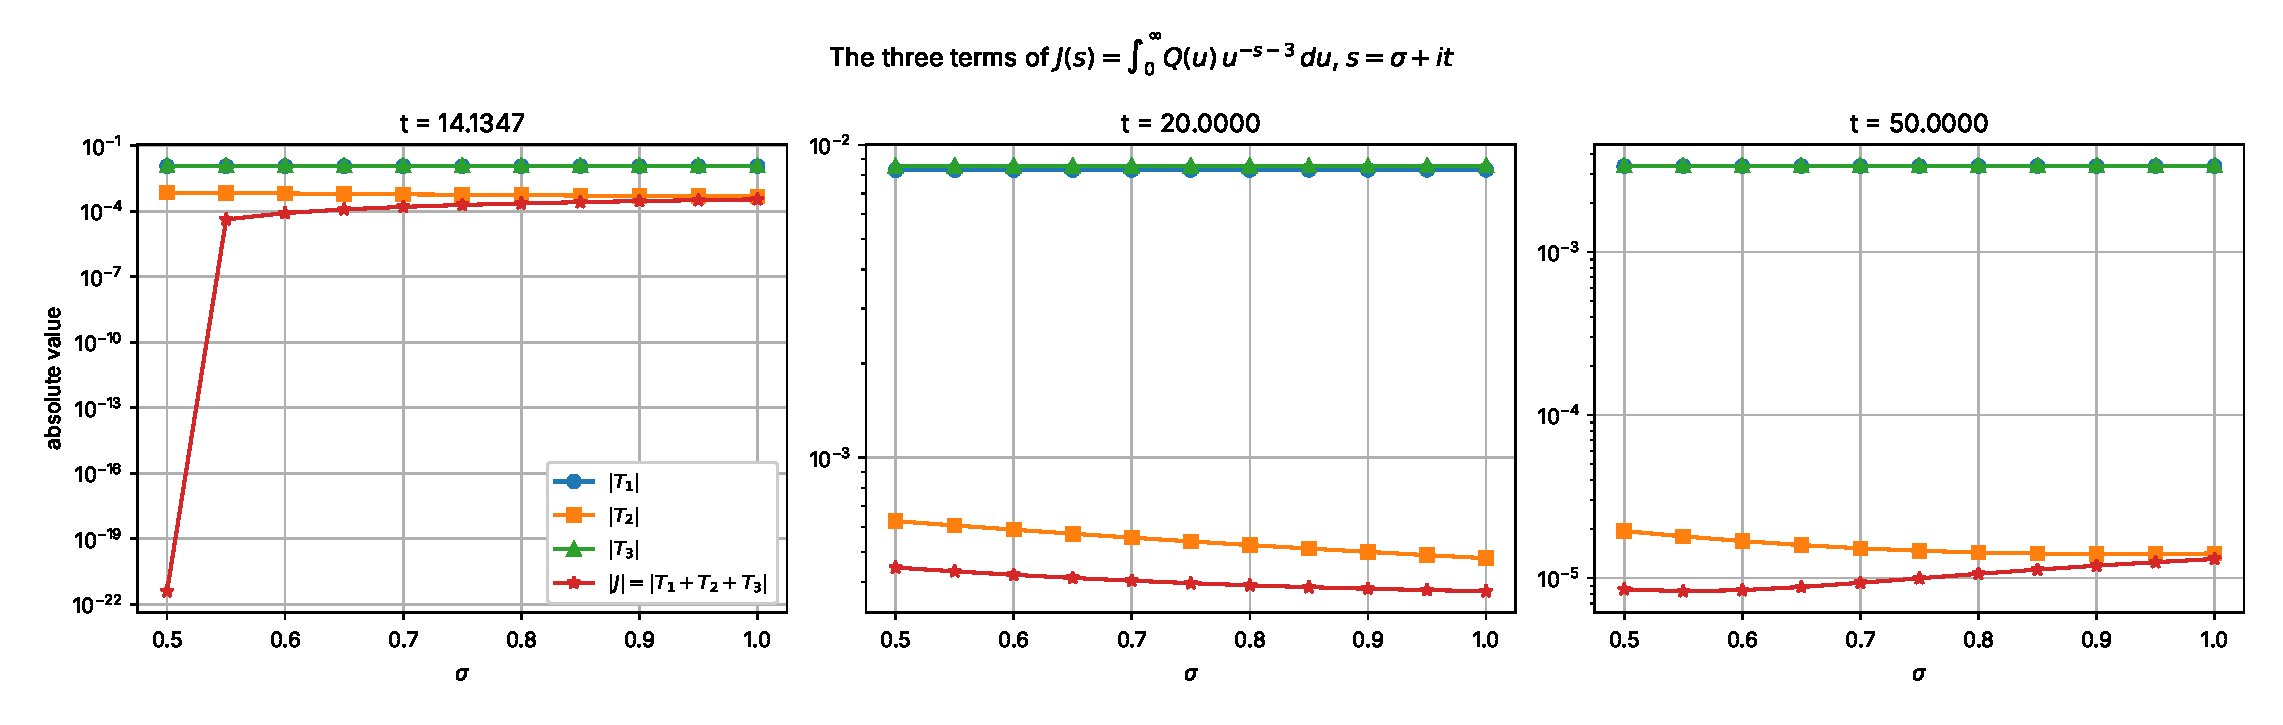
\includegraphics[width=\textwidth]{fig_J_terms_v4.eps}
\caption{$|T_1|$, $|T_2|$, $|T_3|$ and $|J|=|T_1+T_2+T_3|$ against $\sigma\in[\frac12,1]$ at $t=t_1$, $20$, $50$ (logarithmic vertical scale).}\label{fig:J}
\end{figure}

The data show what Corollary~\ref{cor:T13} predicts: $|T_1|$ and $|T_3|$ differ by $6\%$ at $t_1$, $3\%$ at $t=20$ and $0.7\%$ at $t=50$, decrease like $1/t$ ($t|T_3|\approx0.17$ at all three heights, consistent with $|c|/2=0.169$), and are almost independent of $\sigma$. Thus $J$ is the sum of $T_2$ and $T_1+T_3$, which are of comparable size, and $J(s)=0$ if and only if $T_2(s)=-(T_1(s)+T_3(s))$.

\begin{thebibliography}{99}\raggedright

\bibitem{Adam2020}
A.~Adam,
\emph{Generalized hypergeometric expansion related to the Hurwitz zeta function},
preprint (2020); \href{https://arxiv.org/abs/2009.07134}{arXiv:2009.07134}

\bibitem{Alkan2013}
E.~Alkan,
\emph{Approximation by special values of harmonic zeta function and log-sine integrals},
Commun.\ Number Theory Phys.\ \textbf{7} (2013)

\bibitem{BorweinStraub2012}
J.~M.~Borwein and A.~Straub,
\emph{Log-sine evaluations of Mahler measures},
J.\ Aust.\ Math.\ Soc.\ \textbf{92} (2012), 15--36;
\href{https://doi.org/10.1017/S1446788712000067}{doi:10.1017/S1446788712000067}

\bibitem{ChoiChoSrivastava2009}
J.~Choi, Y.~J.~Cho and H.~M.~Srivastava,
\emph{Log-sine integrals involving series associated with the zeta function and polylogarithms},
Math.\ Scand.\ \textbf{105} (2009), 199--217;
\href{https://doi.org/10.7146/math.scand.a-15115}{doi:10.7146/math.scand.a-15115}

\bibitem{Fuchs2025}
S.~Fuchs,
\emph{Fej\'er-kernel prime indicators},
preprint (2025); \href{https://arxiv.org/abs/2506.18933}{arXiv:2506.18933}

\bibitem{Hilberdink2011}
T.~Hilberdink,
\emph{Flows of Mellin transforms with periodic integrator},
J.\ Th\'eor.\ Nombres Bordeaux \textbf{23} (2011), 455--469;
\href{https://doi.org/10.5802/jtnb.771}{doi:10.5802/jtnb.771}

\bibitem{KanemitsuYoshimoto1996}
S.~Kanemitsu and M.~Yoshimoto,
\emph{Farey series and the Riemann hypothesis},
Acta Arith.\ \textbf{75} (1996), 351--374;
\href{https://doi.org/10.4064/aa-75-4-351-374}{doi:10.4064/aa-75-4-351-374}

\bibitem{Kellerhals1995}
R.~Kellerhals,
\emph{Volumes in hyperbolic $5$-space},
Geom.\ Funct.\ Anal.\ \textbf{5} (1995), 640--667;
\href{https://doi.org/10.1007/BF01902056}{doi:10.1007/BF01902056}

\bibitem{Koblitz1983}
N.~Koblitz,
\emph{$p$-adic eigen-functions for Kubert distributions},
Canad.\ J.\ Math.\ \textbf{35} (1983), no.~4, 674--686;
\href{https://doi.org/10.4153/CJM-1983-038-8}{doi:10.4153/CJM-1983-038-8}

\bibitem{KMW2007}
N.~Kurokawa, K.~Mimachi and M.~Wakayama,
\emph{Jackson's integral of the Hurwitz zeta function},
Rend.\ Circ.\ Mat.\ Palermo (2) \textbf{56} (2007), 43--56;
\href{https://doi.org/10.1007/BF03031427}{doi:10.1007/BF03031427}

\bibitem{LagariasLi2016}
J.~C.~Lagarias and W.-C.~W.~Li,
\emph{The Lerch zeta function IV. Hecke operators},
Res.\ Math.\ Sci.\ \textbf{3} (2016), Art.~33;
\href{https://arxiv.org/abs/1511.08116}{arXiv:1511.08116}

\bibitem{Lewin1981}
L.~Lewin,
\emph{Polylogarithms and Associated Functions}, North-Holland, New York--Amsterdam, 1981

\bibitem{Milnor1983}
J.~Milnor,
\emph{On polylogarithms, Hurwitz zeta functions, and the Kubert identities},
Enseign.\ Math.\ (2) \textbf{29} (1983), 281--322; Zbl~0557.10031

\bibitem{DLMF}
\emph{NIST Digital Library of Mathematical Functions}, Release 1.2.4, F.~W.~J.~Olver et al.\ (eds.), \url{https://dlmf.nist.gov/5.11} (accessed 15 November 2026)

\bibitem{Oberhettinger1974}
F.~Oberhettinger,
\emph{Tables of Mellin Transforms}, Springer, Berlin, 1974;
\href{https://doi.org/10.1007/978-3-642-65975-1}{doi:10.1007/978-3-642-65975-1}

\bibitem{OEIS}
OEIS Foundation Inc.,
\emph{The On-Line Encyclopedia of Integer Sequences}, sequence A402034 (allocated),
\url{https://oeis.org/A402034} (accessed 15 November 2026)

\bibitem{Olver1997}
F.~W.~J.~Olver,
\emph{Asymptotics and Special Functions}, A K Peters, Wellesley MA, 1997 (reprint of the 1974 edition)

\bibitem{Onodera2011}
K.~Onodera,
\emph{Generalized log sine integrals and the Mordell--Tornheim zeta values},
Trans.\ Amer.\ Math.\ Soc.\ \textbf{363} (2011), 1463--1485;
\href{https://doi.org/10.1090/S0002-9947-2010-05176-1}{doi:10.1090/S0002-9947-2010-05176-1}

\bibitem{Patri2013}
S.~Patr\`i,
\emph{Sum of the generalized harmonic series with even natural exponent},
Rend.\ Mat.\ Appl.\ (7) \textbf{33} (2013), 19--26

\bibitem{Porubsky2000}
\v{S}.~Porubsk\'y,
\emph{Covering systems, Kubert identities and difference equations},
Math.\ Slovaca \textbf{50} (2000), 381--413; Zbl~0991.11005,
\url{http://dml.cz/dmlcz/136785}

\bibitem{Shalev2025}
N.~Shalev,
\emph{Closed-form evaluations of log-sine integrals and Ap\'ery-like sums in terms of polylogarithms},
preprint; \href{https://arxiv.org/abs/2508.05770}{arXiv:2508.05770}

\bibitem{Titchmarsh1939}
E.~C.~Titchmarsh,
\emph{The Theory of Functions}, 2nd ed., Oxford University Press, Oxford, 1939

\bibitem{TitchmarshHB1986}
E.~C.~Titchmarsh,
\emph{The Theory of the Riemann Zeta-Function}, 2nd ed., revised by D.~R.~Heath-Brown, Oxford University Press, Oxford, 1986

\bibitem{Umezawa2019}
R.~Umezawa,
\emph{Multiple zeta values and iterated log-sine integrals},
preprint (2019); \href{https://arxiv.org/abs/1904.09717}{arXiv:1904.09717}

\bibitem{Zagier2006}
D.~Zagier,
\emph{The Mellin transform and related analytic techniques},
Appendix to E.~Zeidler, \emph{Quantum Field Theory I: Basics in Mathematics and Physics}, Springer, Berlin, 2006, 305--323

\bibitem{ZhangWilliams1995}
N.-Y.~Zhang and K.~S.~Williams,
\emph{Values of the Riemann zeta function and integrals involving $\log(2\sinh\frac\theta2)$ and $\log(2\sin\frac\theta2)$},
Pacific J.\ Math.\ \textbf{168} (1995), 271--289;
\href{https://doi.org/10.2140/pjm.1995.168.271}{doi:10.2140/pjm.1995.168.271}

\end{thebibliography}

\end{document}
